\documentclass[12pt,a4paper,times]{scrreprt}


\usepackage[automark,headsepline]{scrlayer-scrpage}
\usepackage{times}
\usepackage{indentfirst}
\usepackage{microtype}
\usepackage{caption}
\usepackage{subcaption}
\usepackage[a4paper,width=160mm,top=25mm,bottom=25mm,bindingoffset=5mm]{geometry}


\clearpairofpagestyles
\cfoot[\pagemark]{\pagemark}
\lehead{\headmark}
\rohead{\headmark}
\pagestyle{scrheadings}

%% Set Indentation levels and vertical space
\setlength{\parindent}{0.5em}
\setlength{\parskip}{0.5em}

%% Specify "Figures" Folder
\usepackage{graphicx}
\graphicspath{ {./Figures/} }

\usepackage[bookmarks=true]{hyperref}

%% Allow LaTeX for abbreviations like e.g and i.e.
\usepackage[abbreviations,british]{foreign}

%% Header and footer%%

\usepackage{fancyhdr}
\pagestyle{fancy}


\fancyhead[HR]{CT6039}
\fancyhead[HC]{\leftmark}
\fancyhead[HL]{Ben Eriksson}

\fancyfoot{}
\fancyfoot[FR]{Page \thepage}
\fancyfoot[FC]{University of Gloucestershire}
\fancyfoot[FL]{May 2020}

\renewcommand{\headrulewidth}{0.5pt}
\renewcommand{\footrulewidth}{0.5pt}

\usepackage{csquotes}% Recommended

\setlength{\headsep}{5pt}


% Bookmarks for Table of Contents for PDF! 
\hypersetup{
	bookmarks=true,    % show bookmarks bar?
	pdftitle={Applying Machine Learning Models in the Classification of Potentially Malicious Code},    % title
	pdfauthor={Ben Eriksson, S1709406},                     % author
	pdfsubject={},                        % subject of the document
	pdfkeywords={TeX, LaTeX, graphics, images}, % list of keywords
	colorlinks=true,       % false: boxed links; true: colored links
	linkcolor=black,       % color of internal links
	citecolor=black,       % color of links to bibliography
	filecolor=black,        % color of file links
	urlcolor=black,        % color of external links
	linktoc=page            % only page is linked
}

\begin{document}

\begin{titlepage}
\begin{center}
	
    \begin{bfseries}
	\LARGE{Applying Machine Learning Models in the Classification of Potentially Malicious Code}
	
	\vspace{2 cm}
	
	
\includegraphics[width=0.4\textwidth]{./Meta/uogcrest.png}
	
	
	\vspace{2 cm}
	Ben Eriksson\\ s1709402\\
	\vspace{2cm}
	{{\Large Dr. Adam Gorine\\Supervisor}}\\
	\vspace{1.5 cm}
	{{\Large Cyber and Computing Security (Bsc. Hons) } \\
	\vspace{1 cm}
	{\Large School of Computing Technology }}
	\vspace{1 cm} \\
	{\Large May 2020 } 
	\end{bfseries}
        
        
    \end{center}
\end{titlepage}

\chapter*{Declaration}
The following research project and associated proposal is the sole production of myself. 
Any documentation associated that is not of my origin, has been correctly cited and credited to the original Author(s). 
Despite the investigation of potentially malicious software, this research project does not infringe upon the ethical research principals outlined in the relevant University of Gloucestershires' Handbook.  
Any potentially malicious code has been legally obtained from the gratuity of Industry experts, whom produce such content for an equal goal of investigate learning within the community.  
Extensive efforts have been made to ensure the collected data remains isolated from any other Information Technology devices that aren't within scope. 


\chapter*{Acknowledgements}
\par I would like to use the opportunity to express my eternal gratitude towards my family and friends for their continued encouragement throughout the course of my Studies at the hardest of times. Moreover, the enthusiasm expressed by Dr. Adam Gorine - my supervisor for this project, has been a great source of corroboration; His expertise has proven to be invaluable for me.

\par
the following research project has required me to take responsibility upon learning an enormous topic that is abroad of my Module choices throughout the Year. The opportunity has brought a new perspective of Cyber Security upon me, and kindled my ability to contribute towards real-world issues. 



\chapter*{Abstract}
The prevalent risk of malicious infection is an ever-increasing threat to the availability of World-wide Information Technology infrastructure, whom form as pillars to day-to-day society as we know it.

Presenting in many forms, Malware variants have a variety of common objectives from an attacker’s perspective. One category known as Ransomware, is a variant of malicious code whom prohibits a User from accessing a system and/or its data until a ransom is paid - a modern twist on the traditional extortion schemes used by criminal syndicates.
This is an especially noticeable limitation in current methodologies for malignant detection, using signature-based detection, which uses pre-determined rule sets to identify code as malignant or not.

The following research project investigates and experiments with applying machine-learning models to be able to score the maliciousness of code within datasets based upon their heuristics, where the models have no prior-knowledge of the file presented.

\renewcommand\contentsname{Table of Contents}
\renewcommand\listfigurename{Table of Figures}
\renewcommand\listtablename{Table of Tables}

\tableofcontents
\listoffigures
\listoftables


\chapter{Introduction}
\thispagestyle{fancy}
%\vspace{-2em}
\section{Overview}

Whilst the idea of combining Computing resources and technical knowledge to solve both human social and scientific issues isn't a new concept, the introduction of Machine Learning and the use of Artificial Intelligence to solve problems of a grandeur scale is at an unprecedented level. 


The applicability of AI can be seen as implemented at all scales of suitability. Companies such as Facebook and Twitter use Artificial Intelligence to learn more about their Users at an individual level, tailoring the content that is delivered that is relevant to their interests. Or from a business perspective, deliver customised advertising that will bring a much higher rate of ad-revenue because of the Users interests.  



Considering, this use of AI is arguably trivial when comparing other implementations of the ground-breaking technology. Ranging from self-driving Cars to progressing the very forefront of Science with Quantum Computing and bio-medical prediction. (Chui et al., 2019), 
This research project will investigate and apply various machine-learning algorithms and models against a collated data-set of Portable Executable's, henceforth referenced as PE files for identification of their behaviour and intent to a host Operating System  
Microsoft Windows’ PE file is a standard of file-formatting, insisting the structure of various objects across the family of Windows Operating System releases.  



This PE structure is a prevalent rule-set that can be found across many file-types; ranging from executable files for applications, to text-font files and object files - all essential for functionality of the Operating System.  
The Windows PE File comprises of eleven sections. Whilst application Authors can populate these sections as desired, each section will contain metadata, informing the Operating System of how the file should be processed within the application (e.g. defining it as a executable file rather than an object file) (Windows Developer Center, 2019). 

Whilst the Windows Operating System family has evolved, the PE file has continued with little variation.

\par

Microsoft's Windows Operating System has done a remarkable job at maintaining compatibility with previous generations of the Windows Operating System. The MS-DOS header within a PE file is an excellent example of these efforts of backwards compatibility. This header enables the Operating System to process the file and check for compatibility across the whole file. Where there is no compatibility, rather than just crashing as the first editions of MS-DOS used too, the Operating System will now just inform the User that there is no current compatibility. 

\newpage

\section{Problem Statement}


This research project will highlight the limitations of current mitigations in place to combat the threat of Malware. Signature-based identification is the first-line of defence against the war on Malware. 
Signature-based protection solely relies upon the malignant intent of a sample file already being identified. This could be through various channels such as manual inspection from an Analyst investigating the files behaviour to the pre-cursor knowledge of the behaviours the file exhibits, i.e. the file has performed malicious actions on a previous device. 
Due to the biological characteristics of malicious code, the identification of brand-new or “zero-day” variants are an on-going "Cat and Mouse" game between both Malware Analyst and Malicious threat actor. These threat actors can create a substrate of a pre-existing Malware variant in very little time - in comparison to the resources needed for a Malware Analyst to determine the heuristics and behaviours of such generated code. 
As Signature-based detection effectively compares a file’s “fingerprint” or signature against a predetermined list. These signatures are created from a bit-to-bit accuracy, where any deviation of for example, a character will attribute the file with a new signature. This is extremely problematic in combatting Malware, as although the malicious intent of the file remains the same, due to fact there is a slight deviation, an anti-virus engine using Signature-based detection will treat it as a safe file. 


In the context of Artificial Intelligence, classification is a quintessential concept. From detecting animals to the likes of human expression. The proposed research project explores pre-existing classification concepts to create an Artificial Intelligence model capable of detecting new substrates of malicious code “on the fly” as opposed to traditional, current capabilities.

\section{Research Questions}


\begin{itemize}
	\item What attributes can be found within malicious code that can be used to identify its intent? 
	\item Do variants of malicious code have similar attributes, and can these common characteristics be applied to the same machine-learning model used for classification?
	\item Can these attribute identification be accurate enough for a true-positive classification, in comparison to traditional methods of classification such as signature-based detection? 
	\item What signatures and characteristics do current Anti-Virus engines use to identify and classify variants of malicious code?
	\item Can any machine-learning model be used to combat never-seen before substrates of malicious code from knowledge of pre-existing Malware?
\end{itemize}

\newpage

\section{Research Objectives}


To achieve the aim laid out for this research project, the following objectives will be investigated:

\begin{table}[!ht]
	\centering
	% To place a caption above a table
	\caption{Defining the Research Objectives of this Paper.}
	\label{table:1}
	\begin{tabular}{lllll}
		\cline{1-2}
		\multicolumn{1}{|l|}{1} & \multicolumn{1}{l|}{\begin{tabular}[c]{@{}l@{}}To investigate the characteristics of malicious code and\\   how these attributes can be used by a Machine Learning model for\\   identification.\end{tabular}}                                                                 &  &  &  \\ \cline{1-2}
		\multicolumn{1}{|l|}{2} & \multicolumn{1}{l|}{\begin{tabular}[c]{@{}l@{}}To assess pre-existing Machine Learning Models and Malware\\   identification techniques and understand their effectiveness in identifying\\   malicious code.\end{tabular}}                                                    &  &  &  \\ \cline{1-2}
		\multicolumn{1}{|l|}{3} & \multicolumn{1}{l|}{\begin{tabular}[c]{@{}l@{}}To evaluate the reliability and accuracy of a variety of\\   developed Machine Learning Models and their performance in detecting\\   malicious heuristics of code, identifying and preventing further infection.\end{tabular}} &  &  &  \\ \cline{1-2}
		&                                                                                                                                                                                                             &  &  & 
	\end{tabular}
\end{table}



\chapter{Methodology}
\thispagestyle{fancy}
\section{Overview}

When trying to solve a problem using Classification, there are two significant algorithmic approaches that are considered, each with beneficiaries and adversaries that may also go hand-in-hand. 

For instance, the approach of using a decision tree-based model for identifying malicious code seems appealing – resembling a flowchart. 
As Figure 4 below shows, a file can be inputted into the algorithm, where it is analysed for certain attributes that have been pre-determined as malignant or not. 

 \begin{figure}[ht]
  	\centering
 	\label{fig1:example-flowchart-dt-ml}
 	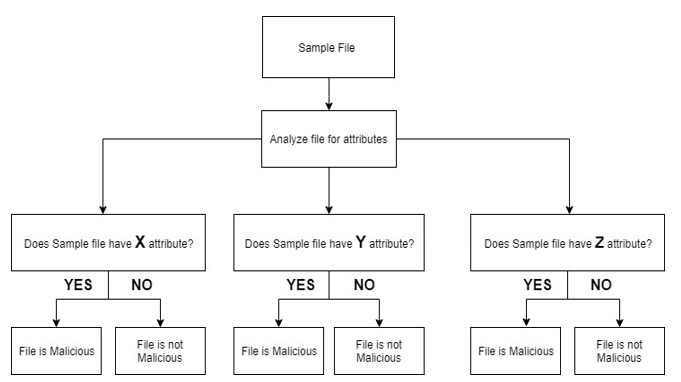
\includegraphics[width=\textwidth]{/Methodology/flowchart-decision-tree}
 	\caption{An example Flowchart illustrating decision-tree based Machine Learning.}
 	
 \end{figure}

\chapter{Literature Review}
\thispagestyle{fancy}
\section{Literature Review}

Malware analysis is a complex and ever-changing topic, containing many features to train a machine learning model upon. As (Schultz et al., 2000) proposes, “Eight to ten malicious programs are created every day, and most cannot be accurately detected until signatures have been generated for them” indicating a huge necessity for real-time analysis to be made to prevent infection on host devices.  
This is supported by Symantec, an industry revolutioniser in commercial Anti-Virus engines, whom report of “[an increase] in the first six months of 2017, Symantec blocked just over 319,000 ransomware infections” (Symantec, 2017) evidently, Malware, especially ransomware is on the dramatic increase. Case studies such as WannaCry “with infections recorded across 150 countries globally” (Nominet, 2017) lightly demonstrate the global and non-target-specific gripe the threat poses. 

  
Thankfully, there has been some continued investigation into circumventing the limitations that signature-based detection retains. For example, (Schultz et al., 2000) created a framework whom “automatically extracted a binary profile from each example in [their] dataset” using “properties … such as byte sequences”. This is an effective alternative to other frameworks proposed by researchers such as (Tesauro, Kephart and Sorkin., 1996) who only achieved a small detection rate due to only investigating PC Boot-sector viruses, of which “PC boot sectors are 512 bytes long”. With this limited amount of code, there is a very minimal expectation of the features that can be extracted.  
When larger datasets containing a lot of features are created, such as that in (Mohaisen, Alrawi and Mohaisen, 2015) Consisting of a much larger scale of “115,157 malware samples”.  


Whilst the study “used only a total of 65 features for classification and clustering”, their best performing algorithm achieved a 85 accuracy rate. However, it should be noted that their performance scale was calculated on both the highest yet most time-efficient algorithm. Other explored frameworks may have achieved a higher accuracy score, however at a much higher systemresource cost.  
This is a noticeable improvement over alternatively suggested frameworks and algorithms such as those of (Bayer et al, 2009), whom suggest that “aggressive approximate clustering techniques may need to be employed [with much larger datasets]” resulting in a loss of accuracy due to generalization. The dramatic decrease in accuracy as cluster – hence dataset sizes increases is shown in Figure 2 


Arguably, system-resource usage is an expendable commodity in order to achieve a higher classification detection rate, especially in a corporate environment. Although, a much larger corporate environment such as an Enterprise who faces a vast quantity of advanced persistent threats from malicious actors daily. 
Binary classification appears to be a popular and successful approach to solving the issue of Malware classification. Binary classification, within the context of extracting information of Malware involves the “process of classifying given document/account on the basis of predefined classes” (Kumari and Kr., 2017). 


\end{document} 